
\section{Machine Learning Experiments}\label{sec:ml_exp}
In this section, we will provide an overview of two machine learning experiments pertinent to the two research questions \ref{sec:introduction}.
The first experiment aims to examine the effectiveness of an XGBoost model in predicting pointing scan offsets to enhance the pointing accuracy.
The primary objective of this experiment is to assess whether the proposed model can outperform the current model in terms of pointing accuracy.
The second experiment aims to investigate the effectiveness of neural networks in developing a pointing model that could replace the current linear model, which is created through linear regression.
It explores the feasibility of a more sophisticated model in terms of pointing accuracy.

\subsection{Experiment 1: Pointing Correction Model} \label{sec:exp1}
This experiment aims to improve the accuracy of the existing pointing model by training XGBoost models to predict offsets obtained from pointing scans.
To accomplish this, we utilized two different datasets, which we processed using the cleaning outlined in section \ref{sec:cleaning_pt_scan}.
The difference between these datasets is that one contains the scans from all instruments, while the other only contains the scans from NFLASH230.
By training our models on these datasets, we aim to reduce the pointing offset and improve the accuracy of the pointing.
In addition, we varied the way we split the datasets for training and testing.
We considered two cases:

\begin{itemize}
    \item \textbf{Case 1:} The dataset is sorted by date and split into six equal-sized folds.
    We consider each of the folds one by one.
    For each of these folds, we use the last $1/6$th of the data as a test set and the remaining $5/6$th as training and validation.
    \item \textbf{Case 2:} The dataset is sorted by date and split into six equal-sized folds.
    We used $5/6$ of the data for training and validation and the remaining for testing.
    We repeated this process six times, using each fold for testing once.
\end{itemize}

Figure \ref{fig:datasplit_cases} illustrates the two cases.
In both cases, we trained and validated the model on $5/6$ of the data and tested on the last $1/6$.
The difference is the amount of data used for training, which can indicate whether models trained on shorter or longer periods perform better.
Using longer period, and thus more data, can help the model find complex relations.
However, a smaller period may be better for learning relations that change over time, as we would expect less variation in a shorter period.

We also split the training and validation data such that scans from a given day only can be either in the training or validation set, not both.
When splitting the data, we used $35\%$ of the days for validation and $65\%$ for training.
This does not amount to precisely the same percentage of scans for the given split, but something close to it nonetheless.


\begin{figure}[H]
    \centering
    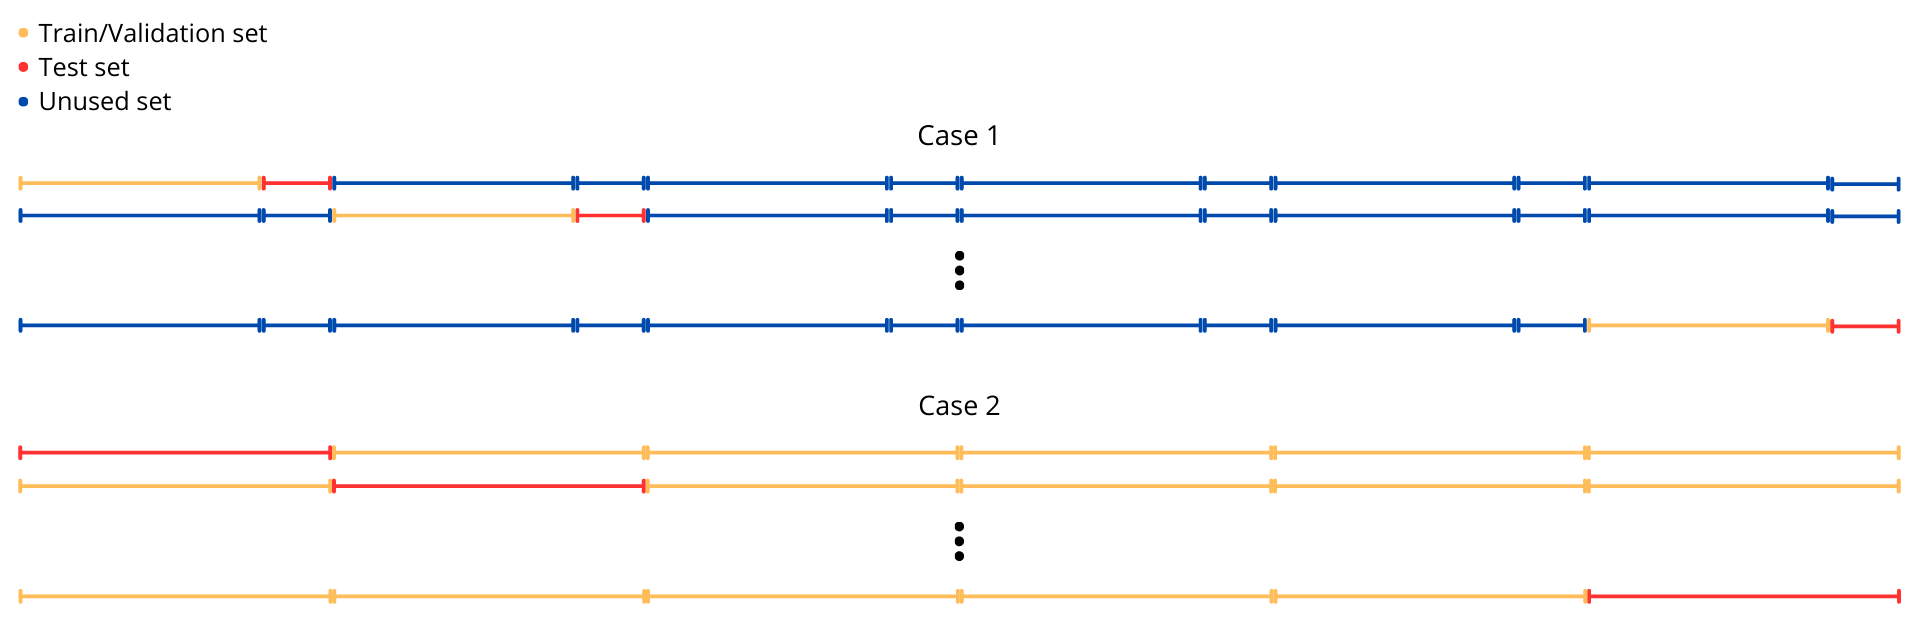
\includegraphics[width=0.98\textwidth]{Canva/datasplits.png}
    \caption{This figure shows two cross-validation cases: the orange region represents the train and validation set, the red region represents the test set, and the blue region is unused for evaluation.
    In \textbf{Case 1}, the dataset is split into six equal-sized folds sorted by date.
    For the selected fold, we use the last part (colored red) for testing and the remaining part (colored orange) for training and validation.
    This process is repeated six times, once for each fold.
    In \textbf{Case 2}, the dataset is again split into six equal-sized folds sorted by date.
    However, we use one whole fold for testing this time and the remaining five for training and validation.
    This process is repeated six times, with each fold used exactly once for testing.}
    \label{fig:datasplit_cases}
\end{figure}




\subsubsection{Feature Selection}
We trained models using a range of features, specifically $k=[2,5,10,20,30,40,50]$ features.
We selected the $k$ features that had the greatest mutual information for each model with the target value.
This approach helps us identify the most important features to improve the model's performance. Selecting a subset of features can reduce the noise in the data. 
By selecting different numbers of features, we can explore the trade-off between model complexity and performance.\textcolor{red}{write and ref to mutual info in theory section}.

\subsubsection{Model Architecture}
We performed a Bayesian hyperparameter search for each model using the parameter space in Table \ref{tab:xgb_hyperparameters_pcorr}.
The search space includes eight hyperparameters that affect the model's complexity, such as the maximum depth of the trees, the regularization strength, and the learning rate.
We used a uniform or log-uniform distribution to sample each hyperparameter within a specific range.
We evaluated $200$ different combinations of hyperparameters (for each dataset, cross-validation case, target variable, and the number of features selected) to find the optimal values for each model.
The models were validated using the MSE, and we picked the model with the best performance on the validation set.


\begin{table}[H]
    \centering
    \caption{This table presents a list of parameters we sampled during hyperparameter tuning for the pointing correction model. The table includes names, sampled distributions, and corresponding ranges.}
    \begin{tabular}{lcc}
        \toprule
        \textbf{Parameter} & \textbf{Sample Distribution} & \textbf{Range} \\ \hline
        max depth & Uniform & [$1$, $5$] \\ 
        reg lambda & Uniform & [$0$, $1$] \\ 
        colsample bytree & Uniform & [$0.5$, $1$] \\ 
        n estimators & Uniform & [$20$, $500$] \\ 
        learning rate & Log-Uniform & [$10^{-5}$, $1$] \\ 
        subsample & Uniform & [$0.5$, $1$] \\ 
        gamma & Log-Uniform & [$10^{-5}$, $1$] \\ 
        min child weight & Uniform & [$1$, $10$] \\ 
        \bottomrule
    \end{tabular}
    \label{tab:xgb_hyperparameters_pcorr}
\end{table}



\subsubsection{Model Evaluation}
To evaluate the performance of the models, we calculated the RMS on each test fold and compared it to the current RMS of the telescope on the same data.
The RMS is calculated for azimuth and elevation separately since an XGBoost model only can predict one target.
For a fold $j$ and target either azimuth or elevation, we calculate the RMS by
\begin{equation}
    RMS_{\text{target},j} = \sqrt{\frac{1}{N_j}\sum_{i=1}^{N_j} (\tilde{\delta}_{\text{target},ji} - \delta_{\text{target},ji})^2},
\end{equation}
where $\tilde{\delta}_{\text{target},ji}$ is the predicted pointing offset and $\delta_{\text{target},ji}$ is the true pointing offset for the $i$th pointing scan in fold $j$.
$N_j$ is the number of pointing scans in fold $j$. 
We then computed the ratio $r_{RMS,j}$ of the model's RMS to the current RMS for each fold.
If the ratio is less than $1$, it indicates that the XGBoost model provides an improvement over the current performance of the telescope for a given fold.

To obtain an overall measure of the model's performance compared to the current performance of the telescope, we averaged the ratios $r_{RMS,j}$ over all six test folds
\begin{equation} \label{eq:mean_rms_compared}
    \bar{r}_{RMS} = \sum_{i=1}^6 \frac{RMS_{model,j}}{RMS_{current,j}}.
\end{equation}
This gives us an average ratio $\bar{r}_{RMS}$, which measures the improvement in performance provided by the XGBoost model.
If $\bar{r}_{RMS} < 1$, it indicates that the XGBoost model outperforms the current pointing correction method on average across all test folds.
By comparing the average ratio $\bar{r}_{RMS}$ for the two different cross-validation cases in Figure \ref{fig:datasplit_cases} and the selected number of features,
we can identify which models provide the best performance.



\subsection{Experiment 2: Pointing Model using Neural Networks}
This experiment uses the raw dataset containing input coordinates, $Az_{\text{input}}$ and $El_{\text{input}}$ respectively, and corresponding true observed values $Az_{\text{observed}}$ and $El_{\text{observed}}$.

The goal is to find a model $f$ such that
\begin{equation}
    f(X) \approx (\delta_{\text{Az}}, \delta_{\text{El}}) = (Az_{\text{observed}}-Az_{\text{input}}, El_{\text{observed}}-El_{\text{input}})
\end{equation}

We split the data into a train, validation, and test set.
The last $15\%$ of the data, which we sorted by date, is used for testing.
We use the remaining $85\%$ of the data for training and validation and split this set into $20\%$ for training and $80\%$ for validation.
This results in $\approx 76\%$ and $\approx 24\%$ of the total dataset used for training and validation.

\subsubsection{Feature Selection}
Selecting the right features is essential in improving the pointing model's accuracy.
This model uses two types of features: geometrical and harmonic terms (some of which are part of the current analytical pointing model [\eqref{eq:analytical_az},\eqref{eq:analytical_el}]) and new features extracted from the telescope's database.
We identified relevant features by calculating Pearson's and Spearman's rank correlation to the offsets for all features.
We analyzed the correlation of the geometrical and harmonic terms using sine and cosine functions of azimuth and elevation up to the fifth order.
Then, we chose the terms with the strongest correlation to the model and used them in all models.
Tables \ref{tab:raw_data_pearson} and \ref{tab:raw_data_spearmans} show the list of features we extracted from the database with a correlation equal to or greater than 0.1.
During model training, we randomly selected a subset of 2 to 19 features from these lists and used them to train the model.
This way of choosing features does not consider complex dependencies between the features that can affect the offsets.
However, training neural networks is computationally heavy, so we must carefully select the features we test.

\subsubsection{Model Architecture}
This experiment utilized four different model architectures.
The first architecture involved feeding all input data into one, two, or three hidden layers.
The other three architectures incorporated machine learning techniques by separating the geometrical and harmonic terms of the input data from the other features and processing them using distinct architectures.
With these approaches, we intend to keep the current model's simplicity and performance while incorporating new features.

The following are the four different architectures:
\begin{enumerate}
    \item \textbf{Regular Neural Network:} All features are passed through the same layers, all with a nonlinear activation function.
    See Figure \ref{subfig:regular}
    \item \textbf{Neural Network with Separated Features 1:} This architecture separates the input features into two groups: geometric and harmonic features and the rest of the features.
    The geometric and harmonic features are connected directly to the linear output layer, while we pass the remaining features through layers with nonlinear activation functions.
    See Figure \ref{subfig:comb_sep1}
    \item \textbf{Neural Network with Separated Features 2:} This architecture is similar to the previous architecture,
    but we feed the geometric and harmonic features through an additional layer of nonlinear activation function before connecting them to the oe utput layer.
    See Figure \ref{subfig:comb_sep2}
    \item \textbf{Neural Network with Separated Features 3:} This architecture combines the previous two architectures by passing the regular features through a few hidden layers with nonlinear activation functions before concatenating them with the geometric and harmonic features.
    We then pass the combined features through a final layer before connecting them to the output layer.
    See Figure \ref{subfig:comb_sep3}
\end{enumerate}
These are visualized in Figure \ref{fig:nn_architecture}.

\begin{figure}[H]
    \centering
    \begin{subfigure}[t]{0.49\textwidth}
        \centering
        % NEURAL NETWORK no text - large
\begin{tikzpicture}[x=2.3cm,y=1.0cm]
  \message{^^JNeural network large}
  \readlist\Nnod{3,4,4,2} % array of number of nodes per layer
  
  \message{^^J  Layer}
  \foreachitem \N \in \Nnod{ % loop over layers
    \def\lay{\Ncnt} % alias of index of current layer
    \pgfmathsetmacro\prev{int(\Ncnt-1)} % number of previous layer
    \message{\lay,}
    \foreach \i [evaluate={\y=\N/2-\i; \x=\lay*0.8; \n=\nstyle;
                           \nprev=int(\prev<\Nnodlen?min(2,\prev):3);}] in {1,...,\N}{ % loop over nodes
      
      % NODES
      %\node[node \n,outer sep=0.6,minimum size=18] (N\lay-\i) at (\x,\y) {};
      \coordinate (N\lay-\i) at (\x,\y);
      
      % CONNECTIONS
      \ifnum\lay>1 % connect to previous layer
        \foreach \j in {1,...,\Nnod[\prev]}{ % loop over nodes in previous layer
          \draw[connect,white,line width=1.2] (N\prev-\j) -- (N\lay-\i);
          \draw[connect] (N\prev-\j) -- (N\lay-\i);
          %\draw[connect] (N\prev-\j.0) -- (N\lay-\i.180); % connect to left
          \node[node \nprev,minimum size=18] at (N\prev-\j) {}; % draw node over lines
        }
        \ifnum \lay=\Nnodlen % draw last node over lines
          \node[node \n,minimum size=18] at (N\lay-\i) {};
        \fi
      \fi % else: nothing to connect first layer
      
    }
  }
  
\end{tikzpicture}
        \caption{\textbf{Regular neural network:}
        This is the standard neural network architecture without any feature separation.
        All features are connected to the same layers.}
        \label{subfig:regular}
    \end{subfigure}
    \hfill
   \begin{subfigure}[t]{0.49\textwidth}
       \centering
       \begin{tikzpicture}[x=2.3cm,y=2.0cm]
  \message{^^JNeural network large}
  \readlist\Nnod{3,2} % array of number of nodes per layer
  \readlist\Nnodtwo{2,3,3,2}
  \message{^^J  Layer}
  \foreachitem \N \in \Nnod{ % loop over layers
    \def\lay{\Ncnt} % alias of index of current layer
    \pgfmathsetmacro\prev{int(\Ncnt-1)} % number of previous layer
    \message{\lay,}
    \foreach \i [evaluate={\y=\N/4-\i*0.5; \x=\lay*0.8+1.6; \n=\nstyle;
                           \nprev=int(\prev<\Nnodlen?min(2,\prev):3);}] in {1,...,\N}{ % loop over nodes
      
      % NODES
      %\node[node \n,outer sep=0.6,minimum size=18] (N\lay-\i) at (\x,\y) {};
      \ifnum \lay<\Nnodlen % draw last node over lines
        \coordinate (N\lay-\i) at (\x,\y);
      \else
        \coordinate (N\lay-\i) at (\x,\y-0.75);
      \fi
      % CONNECTIONS
      \ifnum\lay>1 % connect to previous layer
        \foreach \j in {1,...,\Nnod[\prev]}{ % loop over nodes in previous layer
          \draw[connect,white,line width=1.2] (N\prev-\j) -- (N\lay-\i);
          \draw[connect] (N\prev-\j) -- (N\lay-\i);
          %\draw[connect] (N\prev-\j.0) -- (N\lay-\i.180); % connect to left
          \node[node \nprev,minimum size=18] at (N\prev-\j) {}; % draw node over lines
        }
        \ifnum \lay=\Nnodlen % draw last node over lines
          \node[node \n,minimum size=18] at (N\lay-\i) {};
        \fi
      \fi % else: nothing to connect first layer
      
    }
  }

  \foreachitem \N \in \Nnodtwo{ % loop over layers
    \def\lay{\Ncnt} % alias of index of current layer
    \pgfmathsetmacro\prev{int(\Ncnt-1)} % number of previous layer
    \message{\lay,}
    \foreach \i [evaluate={\y=\N/4-\i*0.5-1.5; \x=\lay*0.8; \n=\nstyle;
                           \nprev=int(\prev<\Nnodtwolen?min(2,\prev):3);}] in {1,...,\N}{ % loop over nodes
      % NODES
      %\node[node \n,outer sep=0.6,minimum size=18] (N\lay-\i) at (\x,\y) {};
      \ifnum \lay<\Nnodtwolen % draw last node over lines
        \coordinate (M\lay-\i) at (\x,\y);
      \else
        \coordinate (M\lay-\i) at (\x,\y+0.75);
      \fi
      % CONNECTIONS
      \ifnum\lay>1 % connect to previous layer
        \foreach \j in {1,...,\Nnodtwo[\prev]}{ % loop over nodes in previous layer
          \draw[connect,white,line width=1.2] (M\prev-\j) -- (M\lay-\i);
          \draw[connect] (M\prev-\j) -- (M\lay-\i);
          %\draw[connect] (N\prev-\j.0) -- (N\lay-\i.180); % connect to left
          \node[node \nprev,minimum size=18] at (M\prev-\j) {}; % draw node over lines
        }
        \ifnum \lay=\Nnodtwolen % draw last node over lines
          \node[node \n,minimum size=18] at (M\lay-\i) {};
        \fi
      \fi % else: nothing to connect first layer
      
    }
  }
  
\end{tikzpicture}
       \caption{\textbf{Neural network with separated features 1:}
       In this architecture, the geometric and harmonic features are separated from the other features and directly connected to the output layer without any nonlinear activation function.}
       \label{subfig:comb_sep1}
\end{subfigure}
\\~\\
    \begin{subfigure}[t]{0.49\textwidth}
        \centering
        \begin{tikzpicture}[x=2.3cm,y=2.0cm]
  \message{^^JNeural network large}
  \readlist\Nnod{3,3,2} % array of number of nodes per layer
  \readlist\Nnodtwo{2,3,3,2}
  \message{^^J  Layer}
  \foreachitem \N \in \Nnod{ % loop over layers
    \def\lay{\Ncnt} % alias of index of current layer
    \pgfmathsetmacro\prev{int(\Ncnt-1)} % number of previous layer
    \message{\lay,}
    \foreach \i [evaluate={\y=\N/4-\i*0.5; \x=\lay*0.8+0.8; \n=\nstyle;
                           \nprev=int(\prev<\Nnodlen?min(2,\prev):3);}] in {1,...,\N}{ % loop over nodes
      
      % NODES
      %\node[node \n,outer sep=0.6,minimum size=18] (N\lay-\i) at (\x,\y) {};
      \ifnum \lay<\Nnodlen % draw last node over lines
        \coordinate (N\lay-\i) at (\x,\y);
      \else
        \coordinate (N\lay-\i) at (\x,\y-0.75);
      \fi
      % CONNECTIONS
      \ifnum\lay>1 % connect to previous layer
        \foreach \j in {1,...,\Nnod[\prev]}{ % loop over nodes in previous layer
          \draw[connect,white,line width=1.2] (N\prev-\j) -- (N\lay-\i);
          \draw[connect] (N\prev-\j) -- (N\lay-\i);
          %\draw[connect] (N\prev-\j.0) -- (N\lay-\i.180); % connect to left
          \node[node \nprev,minimum size=18] at (N\prev-\j) {}; % draw node over lines
        }
        \ifnum \lay=\Nnodlen % draw last node over lines
          \node[node \n,minimum size=18] at (N\lay-\i) {};
        \fi
      \fi % else: nothing to connect first layer
      
    }
  }
  \node[shift = {(-1.5,0)}] at (N2-2){
    $\begin{aligned}
      \text{Geom}&\text{etric}\\
      +&\\
      \text{Harm}&\text{onics}
    \end{aligned}$
  };
  \node[shift = {(-1.5,-0.85)}] at (N2-2){Nonlinear};
  \foreachitem \N \in \Nnodtwo{ % loop over layers
    \def\lay{\Ncnt} % alias of index of current layer
    \pgfmathsetmacro\prev{int(\Ncnt-1)} % number of previous layer
    \message{\lay,}
    \foreach \i [evaluate={\y=\N/4-\i*0.5-1.5; \x=\lay*0.8; \n=\nstyle;
                           \nprev=int(\prev<\Nnodtwolen?min(2,\prev):3);}] in {1,...,\N}{ % loop over nodes
      % NODES
      %\node[node \n,outer sep=0.6,minimum size=18] (N\lay-\i) at (\x,\y) {};
      \ifnum \lay<\Nnodtwolen % draw last node over lines
        \coordinate (M\lay-\i) at (\x,\y);
      \else
        \coordinate (M\lay-\i) at (\x,\y+0.75);
      \fi
      % CONNECTIONS
      \ifnum\lay>1 % connect to previous layer
        \foreach \j in {1,...,\Nnodtwo[\prev]}{ % loop over nodes in previous layer
          \draw[connect,white,line width=1.2] (M\prev-\j) -- (M\lay-\i);
          \draw[connect] (M\prev-\j) -- (M\lay-\i);
          %\draw[connect] (N\prev-\j.0) -- (N\lay-\i.180); % connect to left
          \node[node \nprev,minimum size=18] at (M\prev-\j) {}; % draw node over lines
        }
        \ifnum \lay=\Nnodtwolen % draw last node over lines
          \node[node \n,minimum size=18] at (M\lay-\i) {};
        \fi
      \fi % else: nothing to connect first layer
      
    }
  }
  
\end{tikzpicture}
        \caption{\textbf{Neural network with separated features 2}:
        Similar to the previous architecture, the geometric and harmonic features are separated from the other features.
        However, they are also processed by a nonlinear activation function before being connected to the output layer.}
        \label{subfig:comb_sep2}
    \end{subfigure}
    \hfill
       \begin{subfigure}[t]{0.49\textwidth}
        \centering
        \begin{tikzpicture}[x=2.3cm,y=2.0cm]
  \message{^^JNeural network large}
  \readlist\Nnod{3,3,2} % array of number of nodes per layer
  \readlist\Nnodtwo{2,3,3,2}
  \message{^^J  Layer}
  \foreachitem \N \in \Nnod{ % loop over layers
    \def\lay{\Ncnt} % alias of index of current layer
    \pgfmathsetmacro\prev{int(\Ncnt-1)} % number of previous layer
    \message{\lay,}
    \foreach \i [evaluate={\y=\N/4-\i*0.5; \x=\lay*0.8+0.8; \n=\nstyle;
                           \nprev=int(\prev<\Nnodlen?min(2,\prev):3);}] in {1,...,\N}{ % loop over nodes
      
      % NODES
      %\node[node \n,outer sep=0.6,minimum size=18] (N\lay-\i) at (\x,\y) {};
      \ifnum \lay<\Nnodlen % draw last node over lines
        \coordinate (N\lay-\i) at (\x,\y);
      \else
        \coordinate (N\lay-\i) at (\x,\y-0.75);
      \fi
      % CONNECTIONS
      \ifnum\lay>1 % connect to previous layer
        \foreach \j in {1,...,\Nnod[\prev]}{ % loop over nodes in previous layer
          \draw[connect,white,line width=1.2] (N\prev-\j) -- (N\lay-\i);
          \draw[connect] (N\prev-\j) -- (N\lay-\i);
          %\draw[connect] (N\prev-\j.0) -- (N\lay-\i.180); % connect to left
          \node[node \nprev,minimum size=18] at (N\prev-\j) {}; % draw node over lines
        }
        \ifnum \lay=\Nnodlen % draw last node over lines
          \node[node \n,minimum size=18] at (N\lay-\i) {};
        \fi
      \fi % else: nothing to connect first layer
      
    }
  }

  \foreachitem \N \in \Nnodtwo{ % loop over layers
    \def\lay{\Ncnt} % alias of index of current layer
    \pgfmathsetmacro\prev{int(\Ncnt-1)} % number of previous layer
    \message{\lay,}
    \foreach \i [evaluate={\y=\N/4-\i*0.5-1.5; \x=\lay*0.8; \n=\nstyle;
                           \nprev=int(\prev<\Nnodtwolen?min(2,\prev):3);}] in {1,...,\N}{ % loop over nodes
      % NODES
      %\node[node \n,outer sep=0.6,minimum size=18] (N\lay-\i) at (\x,\y) {};
      \ifnum \lay<\Nnodtwolen % draw last node over lines
        \coordinate (M\lay-\i) at (\x,\y);
      \else
        \coordinate (M\lay-\i) at (\x,\y+0.75);
      \fi
      % CONNECTIONS
      \ifnum\lay>1 % connect to previous layer
        \foreach \j in {1,...,\Nnodtwo[\prev]}{ % loop over nodes in previous layer
          \draw[connect,white,line width=1.2] (M\prev-\j) -- (M\lay-\i);
          \draw[connect] (M\prev-\j) -- (M\lay-\i);
          %\draw[connect] (N\prev-\j.0) -- (N\lay-\i.180); % connect to left
          \node[node \nprev,minimum size=18] at (M\prev-\j) {}; % draw node over lines
        }
        \ifnum \lay=\Nnodtwolen % draw last node over lines
          \node[node \n,minimum size=18] at (M\lay-\i) {};
        \fi
      \fi % else: nothing to connect first layer
      
    }
  }

  \foreachitem \N \in \Nnod{ % loop over layers
    \def\lay{\Ncnt} % alias of index of current layer
    \pgfmathsetmacro\prev{int(\Ncnt-1)} % number of previous layer
    \message{\lay,}
    \foreach \i [evaluate={\y=\N-\i*0.5; \x=\lay; \n=\nstyle;
                           \nprev=int(\prev<\Nnodlen?min(2,\prev):3);}] in {1,...,\N}{ % loop over nodes
      
      % CONNECTIONS
      \ifnum\lay=2 % connect to previous layer
        \foreach \j in {1,...,\Nnod[\prev]}{ % loop over nodes in previous layer
          \draw[connect,white,line width=1.2] (M3-\j) -- (N\lay-\i);
          \draw[connect] (M3-\j) -- (N\lay-\i);
          %\draw[connect] (N\prev-\j.0) -- (N\lay-\i.180); % connect to left
          \message{^^J Nprev \nprev}
          \node[node 2,minimum size=18] at (M3-\j) {}; % draw node over lines
          \node[node 2,minimum size=18] at (N\lay-\j) {}; % draw node over lines
        }
      \fi % else: nothing to connect first layer
      
    }
  }

  \foreachitem \N \in \Nnodtwo{ % loop over layers
    \def\lay{\Ncnt} % alias of index of current layer
    \pgfmathsetmacro\prev{int(\Ncnt-1)} % number of previous layer
    \message{\lay,}
    \foreach \i [evaluate={\y=\N/4-\i*0.5; \x=\lay+2; \n=\nstyle;
                           \nprev=int(\prev<\Nnodtwolen?min(2,\prev):3);}] in {1,...,\N}{ % loop over nodes
      % NODES
      %\node[node \n,outer sep=0.6,minimum size=18] (N\lay-\i) at (\x,\y) {};
      \ifnum\lay=3 % connect to previous layer
        \foreach \j in {1,...,\Nnodtwo[\prev]}{ % loop over nodes in previous layer
          \message{^^J \lay Here (N1-\j) {l\lay}}
          \draw[connect,white,line width=1.2] (N1-\j) -- (M\lay-\i);
          \draw[connect] (N1-\j) -- (M\lay-\i);
          %\draw[connect] (N\prev-\j.0) -- (N\lay-\i.180); % connect to left
          \node[node 1,minimum size=18] at (N1-\j) {}; % draw node over lines
          \node[node 2,minimum size=18] at (M\lay-\j) {}; % draw node over lines
          
        }

      \fi % else: nothing to connect first layer
      
    }
  }



\end{tikzpicture}
        \caption{\textbf{Neural network with separated features 3:}
        In this architecture, we concatenate the processed regular features to the geometric and harmonic features before being connected to the output layer.}
        \label{subfig:comb_sep3}
    \end{subfigure}
     \caption{These architectures were used to train a base pointing model on raw data.}
     \label{fig:nn_architecture}
\end{figure}

The hyperparameters for the neural networks were randomly sampled from different distributions, as presented in Table \ref{tab:nn_hyperparameters}.
Some parameters were consistent across all models, such as the Adam optimization algorithm and the mean squared error loss function.
In total, we trained $100$ networks of each architecture for $200$ epochs.
We pick the model from the epoch with the best performance on the validation set.
\begin{table}[H]
    \centering
    \caption{This table presents a list of parameters we sampled during hyperparameter tuning for the base pointing model. The table includes names, the distribution we sampled from, and corresponding ranges.}
    \begin{tabular}{lcc}
    \hline
    \textbf{Name} & \textbf{Distribution Type} & \textbf{Range} \\ \hline
    hidden layers & uniform integer & [$1$,$3$] \\
    hidden layer size & uniform integer & [$20$, $120$] \\
    learning rate & uniform & [$0.001$, $0.02$] \\
    batch size & uniform integer & [$32$, $512$] \\
    activation & categorical & [gelu, tanh] \\ \hline
    \end{tabular}
    \label{tab:nn_hyperparameters}
    \end{table}

\subsubsection{Loss Function and Model Evaluation}
To evaluate the performance of the models, we used the root mean squared (RMS), measured in arcseconds, on the test set.
We calculate the RMS as follows:
\begin{equation}
    \text{RMS} = \sqrt{ \frac{1}{N} \sum_{i=1}^N \left( (\tilde{\delta}_{Az,i} - \delta_{Az,i})^2 + (\tilde{\delta}_{El,i} - \delta_{El,i})^2 \right)},
\end{equation}
where $\tilde{\delta}_{Az}$ and $\tilde{\delta}_{El}$ are the predicted offsets, while $\delta_{Az}$ and $\delta_{El}$ are the true values.
$N$ is the number of observations in the test set.

This RMS is used to compare the performance of the models.
It will also be compared with a benchmark linear regression model to see if a machine learning approach offers any improvements.